\documentclass[tikz, border=10pt]{standalone}
\usetikzlibrary{shapes}
\begin{document}
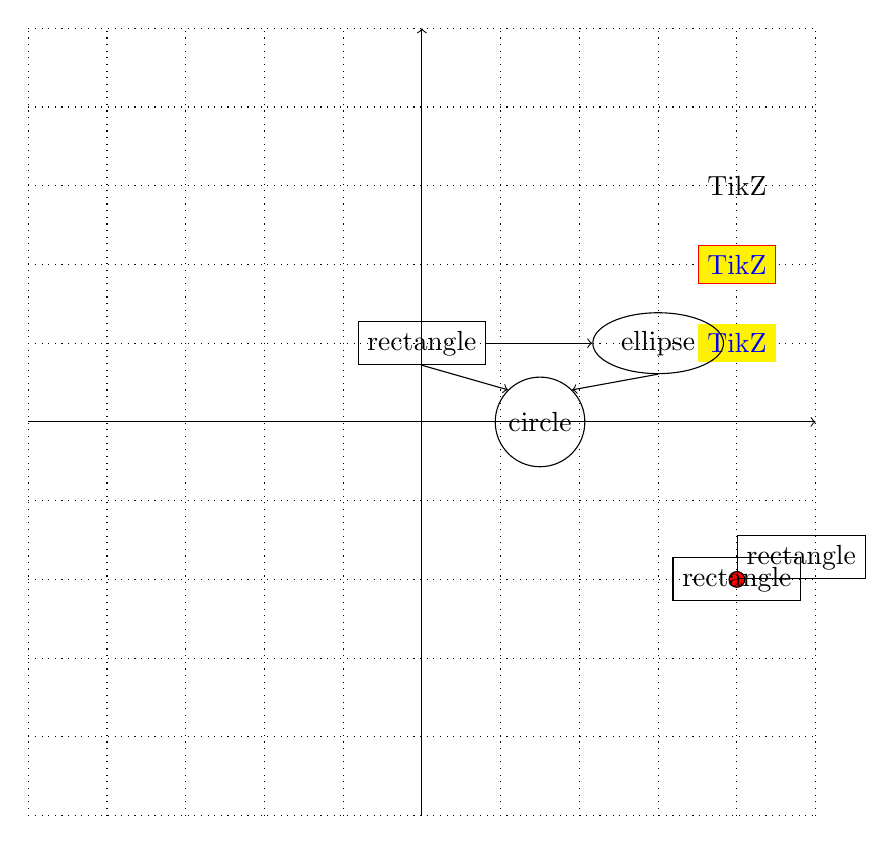
\begin{tikzpicture}
\draw[thin, dotted] (-5, -5) grid[step=1] (5, 5);
\draw[->] (-5, 0)--(5, 0);
\draw[->] (0, -5)--(0, 5);
\draw (4, 3) node {TikZ};
\draw (4, 1) node[color=red, fill=yellow, text=blue] {TikZ};
\draw (4, 2) node[draw, color=red, fill=yellow, text=blue] {TikZ};

\node (r) at (0, 1) [draw, rectangle] {rectangle};
\node (c) at (1.5, 0) [draw, circle] {circle};
\node (e) at (3, 1) [draw, ellipse] {ellipse};

\draw[->] (r.east) -- (e.west);
\draw[->] (r.south) -- (c.north west);
\draw[->] (e.south) -- (c.north east);

\draw[fill=red] (4, -2) circle(0.1);
\node at (4, -2) [draw, rectangle] {rectangle};
\node at (4,-2)[draw, rectangle, anchor=south west]{rectangle};
\end{tikzpicture}
\end{document}